\documentclass[11pt,a4paper]{amsart}
\usepackage[utf8]{inputenc}
\usepackage[T1]{fontenc}
\usepackage[colorlinks=true,citecolor=blue,linkcolor=black]{hyperref}
\usepackage{amsmath,mathtools,amssymb,extarrows,mathrsfs,amsthm}
\usepackage{tikz-cd}
\usepackage{tikz}
\usetikzlibrary{backgrounds}
\usetikzlibrary{calc}
\usetikzlibrary{hobby}
\usetikzlibrary{decorations.markings}
\usetikzlibrary{arrows.meta}
\usepackage{xcolor}

\begin{document}

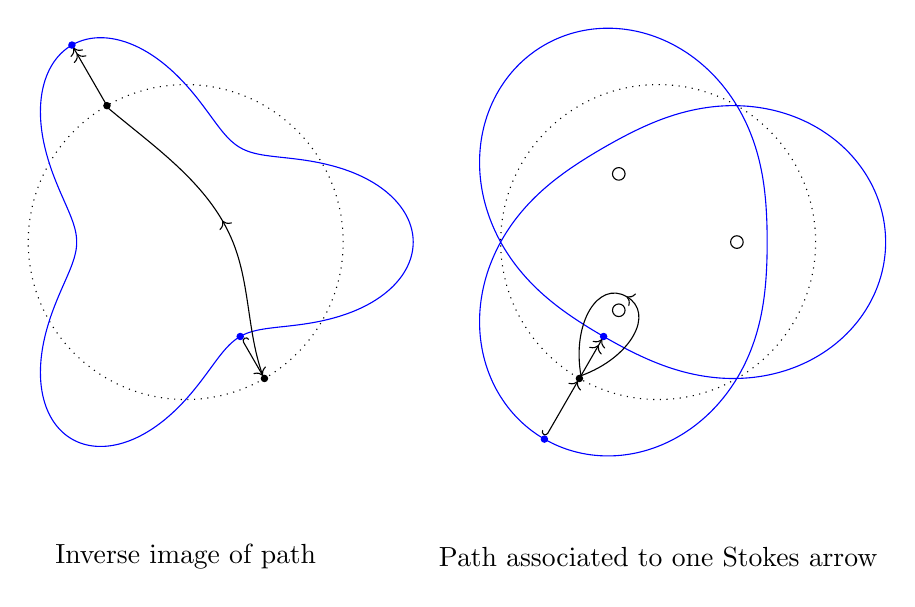
\begin{tikzpicture}[scale=2]
	\begin{scope}
		\draw[dotted] (0,0) circle (1);
		\draw[blue,domain=0:(360),scale=1,samples=1000] plot (\x:{exp(-cos(3*\x+180)/exp(1))}); 
		
		\draw[blue, fill=blue] (-60:{exp(-1/exp(1))}) circle (0.02cm);
		\draw[fill=black] (-60:1) circle (0.02cm);
		\draw[fill=black] (120:1) circle (0.02cm);
		\draw[blue, fill=blue] (120:{exp(1/exp(1))}) circle (0.02cm);
		
		\draw[{Hooks[round,right]}->] (-60:{exp(-1/exp(1))+0.02}) to (-60:0.98); 
		\draw[decoration={markings,mark=at position 0.5 with {\arrow{>}}},postaction={decorate}] (-60:0.98) to [out angle=110, in angle=-40,curve through={(0:0.3)}](120:0.98);
		\draw[->>] (120:0.98) to (120:{exp(1/exp(1))-0.02}); 
		
		\draw (0,-2) node {Inverse image of path};
	\end{scope}
	
	\begin{scope}[xshift=3cm]
		\draw[dotted] (0,0) circle (1);
		\draw[blue,domain=0:(2*360),scale=1,samples=1000] plot (\x:{exp(cos(3/2*\x)/exp(1))}); 
		
		\draw[blue, fill=blue] (-120:{exp(1/exp(1))}) circle (0.02cm);
		\draw[fill=black] (-120:1) circle (0.02cm);
		\draw[blue, fill=blue] (-120:{exp(-1/exp(1))}) circle (0.02cm);
		
		\foreach \th in {0,120,240} \draw (\th:0.5) circle (0.04cm);
		
		\draw[{Hooks[round,right]}->] (-120:{exp(1/exp(1))-0.02}) to (-120:1.02); 
		\draw[decoration={markings,mark=at position 0.5 with {\arrow{>}}},postaction={decorate}] (-120:0.98) to [out angle=20, in angle=100,curve through={(-120:0.4)}](-120:0.98);
		\draw[->>] (-120:1.02) to (-120:{exp(-1/exp(1))+0.02});  
		\draw (0,-2) node {Path associated to one Stokes arrow};
	\end{scope}
\end{tikzpicture}

\end{document}